\documentclass[a4paper]{article}

% --- Packages ---

\usepackage{a4wide}
\usepackage[utf8]{inputenc}
\usepackage{amsmath}
\usepackage{mathtools}
\usepackage{amssymb}
\usepackage[english]{babel}
\usepackage{mdframed}
\usepackage{systeme,}
\usepackage{lipsum}
\usepackage{relsize}
\usepackage{caption}
\usepackage{tikz}
\usepackage{tikz-3dplot}
\usetikzlibrary{shapes.geometric}
\usepackage{pgfplots}
\usepackage{pgfplotstable}
\pgfplotsset{compat=newest}%1.7}
\usepackage{harpoon}%
\usepackage{graphicx}
\usepackage{wrapfig}
\usepackage{subcaption}
\usepackage{authblk}
\usepackage{float}
\usepackage{listings}
\usepackage{xcolor}
\usepackage{chngcntr}
\usepackage{amsthm}
\usepackage{comment}
\usepackage{commath}
\usepackage{hyperref}%Might remove, adds link to each reference
\usepackage{url}
\usepackage{calligra}
\usepackage{pgf}

% --- Bibtex ---

%\usepackage[backend = biblar,]{bibtex}

%\addbibliografy(ref.bib)

% --- Commands --- 

\newcommand{\w}{\omega}
\newcommand{\trace}{\text{Tr}}
\newcommand{\grad}{\mathbf{\nabla}}
%\newcommand{\crr}{\mathfrak{r}}
\newcommand{\laplace}{\nabla^2}
\newcommand{\newparagraph}{\vspace{.5cm}\noindent}

% --- Math character commands ---

\newcommand{\curl}[1]{\mathbf{\nabla}\times \mathbf{#1}}
\newcommand{\dive}[1]{\mathbf{\nabla}\cdot \mathbf{#1}}
\newcommand{\res}[2]{\text{Res}(#1,#2)}
\newcommand{\fpartial}[2]{\frac{\partial #1}{\partial #2}}
\newcommand{\rot}[3]{\begin{vmatrix}\hat{x}&\hat{y}&\hat{z}\\\partial_x&\partial_y&\partial_z\\#1&#2&#3 \end{vmatrix}}
\newcommand{\average}[1]{\langle #1 \rangle}
\newcommand{\ket}[1]{|#1\rangle}
\newcommand{\bra}[1]{\langle #1|}


%  --- Special character commands ---

\DeclareMathAlphabet{\mathcalligra}{T1}{calligra}{m}{n}
\DeclareFontShape{T1}{calligra}{m}{n}{<->s*[2.2]callig15}{}
\newcommand{\crr}{\mathcalligra{r}\,}
\newcommand{\boldscriptr}{\pmb{\mathcalligra{r}}\,}


\title{INPUT TITLE HERE}
\author{Author : Andreas Evensen}
\date{Date: \today}

% --- Code ---

\definecolor{codegreen}{rgb}{0,0.6,0}
\definecolor{codegray}{rgb}{0.5,0.5,0.5}
\definecolor{codepurple}{rgb}{0.58,0,0.82}
\definecolor{backcolour}{rgb}{0.95,0.95,0.92}

\lstdefinestyle{mystyle}{
    backgroundcolor=\color{backcolour},   
    commentstyle=\color{codegreen},
    keywordstyle=\color{magenta},
    numberstyle=\tiny\color{codegray},
    stringstyle=\color{codepurple},
    basicstyle=\ttfamily\footnotesize,
    breakatwhitespace=false,         
    breaklines=true,                 
    captionpos=b,                    
    keepspaces=true,                 
    numbers=left,                    
    numbersep=5pt,                  
    showspaces=false,                
    showstringspaces=false,
    showtabs=false,                  
    tabsize=2
}

\lstset{style=mystyle}

\begin{document}

\thispagestyle{empty}
\begin{titlepage}
   \begin{center}
       % \vspace*{1cm}
       \huge
       \textbf{Molecular dynamics: Argon Fluid}\\
       \vspace*{1cm}
       \textbf{Course: FK8028}
       \large

       \vspace*{0.5cm}
       \textbf{Author: Andreas Evensen}\\
       \vspace*{.5cm}
       \small
       \vspace*{1.cm}
       \textbf{Submission date: \today}\\
       \vspace*{.5cm}
       \vspace{0.8cm}
     
       \small
       Stockholm University\\
       Computational Physics\\
       Sweden\\
   \end{center}
\end{titlepage}

\pagenumbering{Roman}
\newpage
\pagenumbering{roman}
\setcounter{page}{1}
\newpage
\tableofcontents
\newpage
\pagenumbering{arabic}

\section*{Introduction}\addcontentsline{toc}{section}{Introduction}
In this report, the behavior of an NVT ensemble when modeled with Metropolis Monte Carlo, composed of Argon atoms, was investigated. Quantities such as: Potential energy, and position was studied.
The position of the atoms manifested itself in the form of a radial distribution function $g(r)$, which represented the system's probability of finding an atom at a distance $r$ from another atom.
The potential energy of the system was also studied, and the energy of the system was plotted as a function of the number of accepted moves.

\newparagraph
Quantities such as the specific heat capacity $c_v$ was computed, and the result was compared to previously obtained results.
The simulation implemented periodic boundary conditions, and thus effectively simulated an infinite system, in this case liquid Argon.

\section*{Theory \& Method}\addcontentsline{toc}{section}{Theory \& Method}
Monte Carlo simulations are a class of algorithms that can be used to sample a molecular system.
In contrast to molecular dynamics, Monte Carlo simulations do not require the equations of motion to be solved, and thus are computationally less expensive.
This however implies that the Monte-Carlo simulation can not be used to simulate the time evolution of the system but rather the equilibrium state of the system.
The Metropolis Monte Carlo algorithm is specific algorithm that implements detailed balance, which implies balance.
This manifests in the following equation:
\begin{align}
    N(\mathbf{x})\cdot \alpha(\mathbf{x}\to\mathbf{x}') \cdot \beta(\mathbf{x}\to\mathbf{x}') = N(\mathbf{x}')\cdot \alpha(\mathbf{x}'\to\mathbf{x}) \cdot \beta(\mathbf{x}'\to\mathbf{x}).\label{eq: detailed balance}
\end{align}In the above equation, $\mathbf{x}$ is the state of the system and $N(\mathbf{x})$ is the population of state $\mathbf{x}$; the probability function $\alpha$ is probability of receiving a change in state from $\mathbf{x}\to\mathbf{x}'$, whilst the probability function $\beta$ is the probability of accepting such a state.
In Metropolis Monte Carlo, $\alpha(\mathbf{x}\to\mathbf{x}') = \alpha(\mathbf{x}'\to\mathbf{x})$, indicating that the probability of picking an atom is the same, as well as moving it in the same direction. This in itself is achieved by uniform randomness.

\newparagraph
The Metropolis Monte Carlo algorithm is structured in the following manner:
\begin{enumerate}
    \item Pick a random atom
    \item Propose a move
    \item Calculate the change in energy if this move was supposed to occur
    \item Accept or reject the move depending on $\min\left(1, \exp\left[-\beta\Delta E\right]\right)$
    \item Update the system (if move was accepted, otherwise keep the system as it was)
\end{enumerate}This process is repeated for many iterations, such that the system reaches equilibrium.
In contrast to molecular dynamics simulations, the Metropolis Monte Carlo algorithm is faster, it runs in $\mathcal{O}(N)$ time complexity, where $N$ is the number of atoms in the system, per iteration\footnote{In the previously implemented Molecular dynamics simulation, the runtime was $\mathcal{O}(N^2)$ per iteration.}.
Moreover, the Monte Carlo simulation is a stochastic process, and thus the results fluctuate around the true value, even though the system has reached equilibrium.
\newpage

\newparagraph
The radial function distribution, (RDF), $g(r)$ is measurement of the probability of finding an atom at a distance $r$ from another atom, and is defined as
\begin{align}
    g(r_i) = \frac{V}{N}\frac{h(r_i)}{4\pi r_i^2\Delta r}.\label{eq: rdf}
\end{align}The specific heat capacity $c_v$ is defined as:
\begin{align}
    c_v &= \frac{3k_b}{2} - \frac{N\sigma^2(v)}{k_bT^2},\label{eq: specific heat}
\end{align}describes how the energy of the system changes with temperature, and is a measure of the system's ability to store energy. Here $v$ is defined as $\frac{\mathcal{V}}{N}$, where $\mathcal{V}$ is the potential energy and $N$ is the number of atoms.


\section*{Result \& Discussion}\addcontentsline{toc}{section}{Result \& Discussion}
The Monte Carlo simulation was written in V, a static typed compiler language. The simulation ran for $0.5\cdot10^6$ iterations, where the potential energy and the radial function distribution was computed every $1000$ iterations.
This was done to ensure that the system had reached equilibrium, and that the system was ergodic. The temperature was set to $94.4$ K, as this was the temperature at which the system was previously simulated with a Molecular dynamics simulation.
The system was constructed in such a way that the acceptance rate was $28.54$\%. This is close to the target acceptance rate $30$\%.

\newparagraph
The simulation is written in V, and hence, the following random number generator seed was used:
\begin{lstlisting}[language = C, caption = {Random number generator seed}]
    rng: &rand.PRNG(pcg32.PCG32RNG{
    PRNGBuffer: buffer.PRNGBuffer{
        bytes_left: 0
        buffer: 0
    }
    state: 2811831097841394232
    inc: 5511981685926715381
})
\end{lstlisting}

\newparagraph
The radial function distribution $g(r)$ was computed for each for a subset of iterations, and the average of the radial function was plotted in the figure below, fig \ref{fig: radial function}.
\begin{figure}[H]
    \centering
    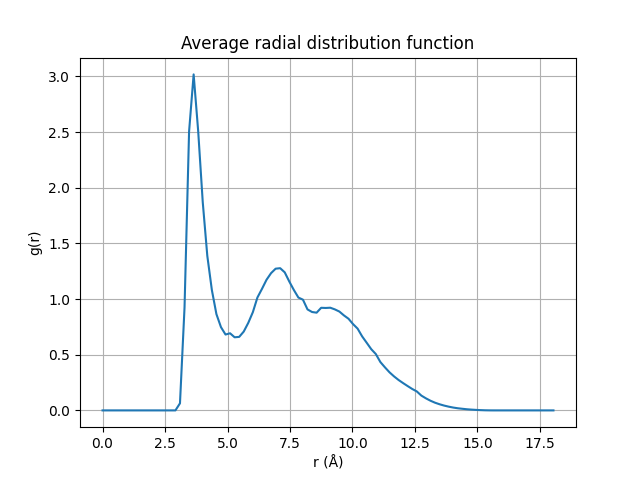
\includegraphics[scale = 0.5]{average_radial.png}
    \caption{Average radial function $g(r)$}
    \label{fig: radial function}
\end{figure}\noindent
The peaks are located around $r = 3.7$~Å, $r=7.3$~Å, and $r = 8.7$~Å, which agrees with preciously found results; the previous results were obtained with a Molecular dynamics simulation.
Since Monte Carlo simulations are stochastic, the RDF fluctuates around the average value, which is given by the ensemble average, since we enforce ergodicity. 
Thus, even though this simulation is computed in the NVT ensemble, the RDF still predicts the same equilibrium state as the molecular dynamics simulation, which predicted an NVE ensemble.

\newparagraph
The potential energy of the system, modeled by a Lennard-Jones potential, was used to model the energy of the system.
If the energy decreased, the move was accepted, and if the energy increased, the move was accepted with a probability $\exp\left[-\beta\Delta E\right]$.
Here $\Delta E$ is the difference in energy between the potential new configuration and the old configuration, and $\beta = \frac{1}{k_bT}$.
The average energy of the system is computed in accordance to:
\begin{align*}
    \average{\mathcal{V}} = \frac{1}{n}\sum_{i=1}^n \mathcal{V}_i,
\end{align*}where $n$ is the number of data points.
This was computed to be: $\average{\mathcal{V}} = -14.80$~eV, which is in agreement with the previously obtained results.
The energy of the system was plotted as a function of the number of accepted moves, and the result is shown in fig \ref{fig: energy}.
\begin{figure}[H]
    \centering
    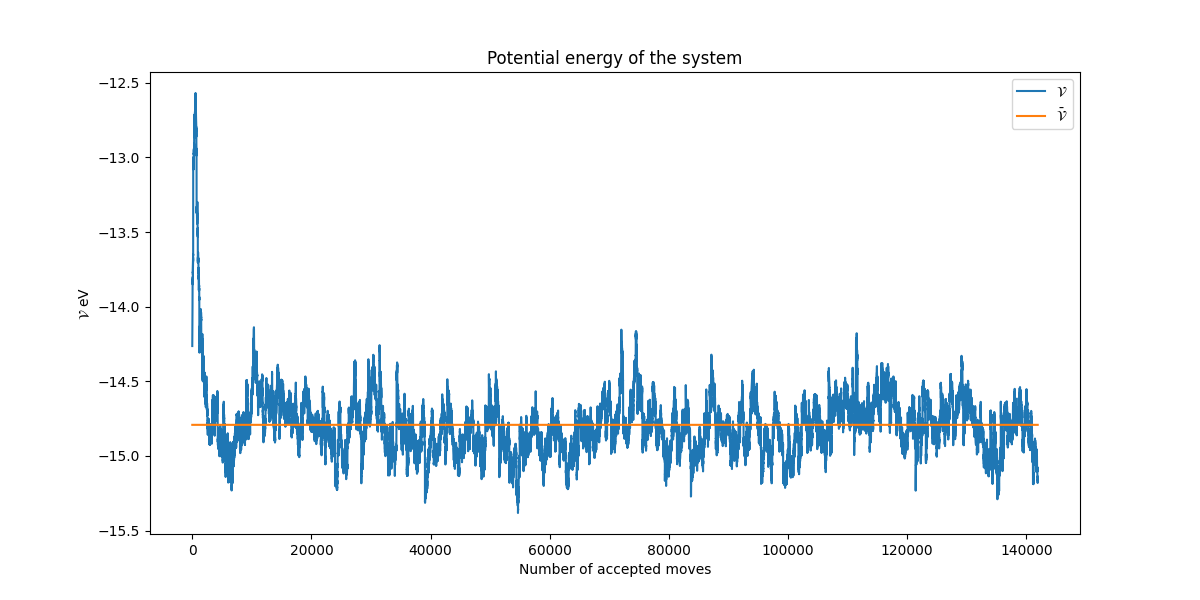
\includegraphics[scale = 0.45]{potential_energy.png}
    \caption{Energy of the system as a function of accepted moves}
    \label{fig: energy}
\end{figure}\noindent
As the number of accepted moves increases, the potential energy quickly equilibrates, and fluctuates around the average value.
To ensure that the system had equilibrated, the block-average method was implemented.
This is shown in the figure below:
\begin{figure}[H]
    \centering
    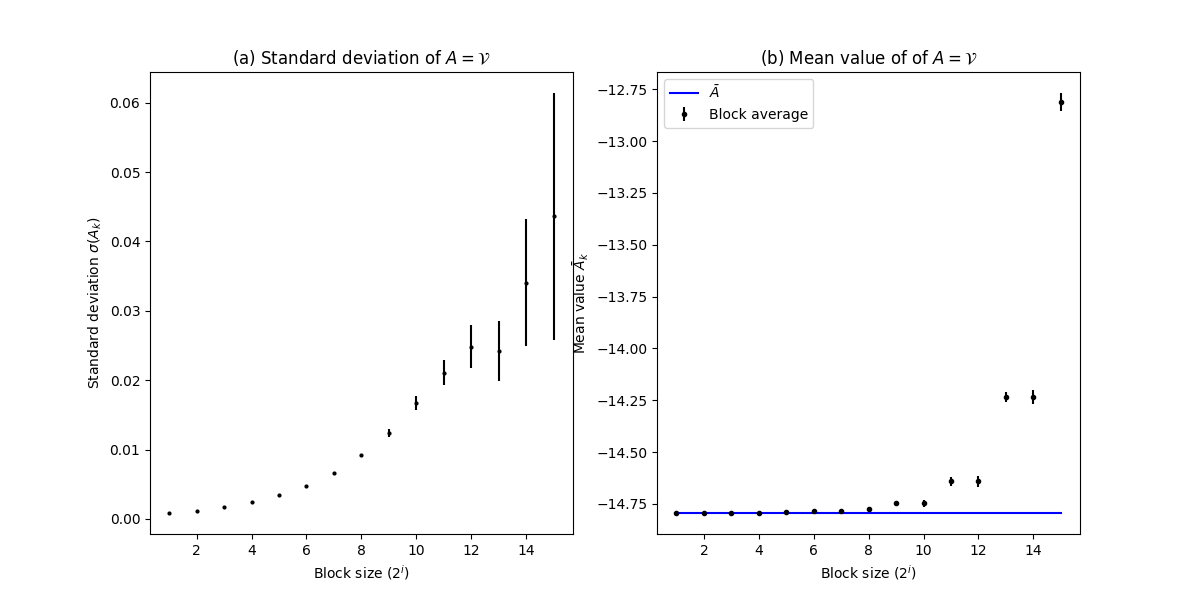
\includegraphics[scale = 0.4]{var_p.png}
    \caption{Block average of the potential energy}
    \label{fig: block average potential}
\end{figure}\noindent
There is a plateau around $2^{15} = 32768$ block length. This indicates that the system has equilibrated, and that the potential energy indeed fluctuates around the true average of the ensemble.
The standard deviation of the potential energy is thus computed to be $\sigma(\mathcal{V}) = 0.23$~eV.
The standard deviation of $\sigma(\bar{\mathcal{V}}) = 0.027$~eV, which is signifcantly smaller.

\newparagraph
The specific heat-capacity is computed in accordance to eq \eqref{eq: specific heat}, and was found to be: $37.75$~J/(K mol).
This result is significantly bigger than the previously obtained result, which was $23.83$~J/(K mol).
This is due to the random number generator used.
Varying the seed of the random number generator, the specific heat capacity fluctuates significantly.

%Even though this is slightly smaller than the previously obtained results, it still agrees with what was found in the previous simulation.

\section*{Conclusion}\addcontentsline{toc}{section}{Conclusion}
The Metropolis Monte Carlo (MC) algorithm implemented agrees with most of the previous found results, even though the MC algorithm modeled a different ensemble (NVT) instead of an NVE ensemble.
The radial function distribution, eq \eqref{eq: rdf}, manifests the same distance between atoms in our MC algorithm as previously found in the molecular dynamics simulation, and the average energy $\average{\mathcal{V}}$ is also in agreement to previous results.
The standard deviation $\sigma(\bar{\mathcal{V}})$ is comparable with the previously found result, but differs with order 10. This is not unexpected since MC is a stochastic process.

\newparagraph
The specific heat capacity $c_v$ differed significantly compared to our molecular dynamics simulation.
As this is a result of the random number generator used, an improvement for future work would be to implement another generator which can provide suitable numbers.


\end{document}
 
